\documentclass[12pt]{article}

\usepackage{amsmath, mathtools}
\usepackage{amsfonts}
\usepackage{amssymb}
\usepackage{graphicx}
\usepackage{colortbl}
\usepackage{xr}
\usepackage{hyperref}
\usepackage{longtable}
\usepackage{xfrac}
\usepackage{tabularx}
\usepackage{float}
\usepackage{siunitx}
\usepackage{booktabs}
\usepackage{caption}
\usepackage{pdflscape}
\usepackage{afterpage}
\usepackage{cool}
\usepackage{comment}
\usepackage{adjustbox}

\restylefloat{table}

\usepackage[round]{natbib}

 

\hypersetup{
    bookmarks=true,         % show bookmarks bar?
    colorlinks=true,       % false: boxed links; true: colored links
    linkcolor=red,          % color of internal links (change box color with linkbordercolor)
    citecolor=green,        % color of links to bibliography
    filecolor=magenta,      % color of file links
    urlcolor=cyan           % color of external links
}

% For easy change of table widths
\newcommand{\colZwidth}{1.0\textwidth}
\newcommand{\colAwidth}{0.13\textwidth}
\newcommand{\colBwidth}{0.82\textwidth}
\newcommand{\colCwidth}{0.1\textwidth}
\newcommand{\colDwidth}{0.05\textwidth}
\newcommand{\colEwidth}{0.8\textwidth}
\newcommand{\colFwidth}{0.17\textwidth}
\newcommand{\colGwidth}{0.5\textwidth}
\newcommand{\colHwidth}{0.28\textwidth}

% Used so that cross-references have a meaningful prefix
\newcounter{defnum} %Definition Number
\newcommand{\dthedefnum}{GD\thedefnum}
\newcommand{\dref}[1]{GD\ref{#1}}
\newcounter{datadefnum} %Datadefinition Number
\newcommand{\ddthedatadefnum}{DD\thedatadefnum}
\newcommand{\ddref}[1]{DD\ref{#1}}
\newcounter{theorynum} %Theory Number
\newcommand{\tthetheorynum}{T\thetheorynum}
\newcommand{\tref}[1]{T\ref{#1}}
\newcounter{tablenum} %Table Number
\newcommand{\tbthetablenum}{T\thetablenum}
\newcommand{\tbref}[1]{TB\ref{#1}}
\newcounter{assumpnum} %Assumption Number
\newcommand{\atheassumpnum}{P\theassumpnum}
\newcommand{\aref}[1]{A\ref{#1}}
\newcounter{goalnum} %Goal Number
\newcommand{\gthegoalnum}{P\thegoalnum}
\newcommand{\gsref}[1]{GS\ref{#1}}
\newcounter{instnum} %Instance Number
\newcommand{\itheinstnum}{IM\theinstnum}
\newcommand{\iref}[1]{IM\ref{#1}}
\newcounter{reqnum} %Requirement Number
\newcommand{\rthereqnum}{P\thereqnum}
\newcommand{\rref}[1]{R\ref{#1}}
\newcounter{lcnum} %Likely change number
\newcommand{\lthelcnum}{LC\thelcnum}
\newcommand{\lcref}[1]{LC\ref{#1}}

\usepackage{fullpage}

\begin{document}

\title{Software Requirements Specification for : \\Double Pendulum} 
\author{Zhi Zhang}
\date{\today}
  
\maketitle

\newpage

\pagenumbering{arabic}

\tableofcontents

\newpage

\section*{Revision History}\label{sec_revision}

\begin{tabularx}{\textwidth}{p{3cm}p{2cm}X}
\toprule {\bf Date} & {\bf Version} & {\bf Notes}\\
\midrule
Oct.02 & 1.0 & Initial Draft\\
\bottomrule
\end{tabularx}


\newpage
\section{Reference Material}\label{sec_ref}

This section records information for easy reference.

\subsection{Table of Units}\label{sec_tableofunits}

Throughout this document SI (Syst\`{e}me International d'Unit\'{e}s) is employed
as the unit system. In addition to the basic units, several derived units are
used as described below. For each unit, the symbol is given followed by a
description of the unit and the SI name.
~\newline

\renewcommand{\arraystretch}{1.2}
\begin{table}[H]
\centering
  \noindent \begin{tabular}{l l l} 
    \toprule    
    \textbf{Symbol} & \textbf{Description} & \textbf{SI Name}\\
    \midrule 
    \si{\kilogram} & mass & kilogram\\
    \si{\second} & time & second\\
    \si{\degree} & angle & degree\\
    \si{\metre} & length & metre\\
    \si{\newton} & force & newton\\
    \bottomrule

  \end{tabular}
  \caption{Table of Units}
\end{table}

\subsection{Table of Symbols}\label{sec_tableofsymbols}

The table that follows summarizes the symbols used in this document along with
their units. The choice of symbols was made to be consistent with the heat
transfer literature and with existing documentation for solar water heating
systems. The symbols are listed in alphabetical order.
~\newline

\renewcommand{\arraystretch}{1.2}
\begin{table}[H]
  \centering
  \noindent \begin{longtable*}{l l p{12cm}} 
  \toprule
  \textbf{symbol} & \textbf{unit} & \textbf{description}\\
  \midrule 
  $x_1$ & \si[per-mode=symbol] {\metre} & horizontal position of the top pendulum 
  \\
  $x_2$ & \si[per-mode=symbol] {\metre} & horizontal position of the bottom pendulum 
  \\
  $y_1$ & \si[per-mode=symbol] {\metre} & vertical position of the top pendulum 
  \\
  $y_2$ & \si[per-mode=symbol] {\metre} & vertical position of the bottom pendulum 
  \\
  ${x_1}'$ & \si[per-mode=symbol] {\metre\per\second} & horizontal velocity of the top pendulum 
  \\
  ${x_2}'$ & \si[per-mode=symbol] {\metre\per\second} & horizontal velocity of the bottom pendulum 
  \\
  ${y_1}'$ & \si[per-mode=symbol] {\metre\per\second} & vertical velocity of the top pendulum 
  \\
  ${y_2}'$ & \si[per-mode=symbol] {\metre\per\second} & vertical velocity of the bottom pendulum 
  \\
  ${x_1}''$ & \si[per-mode=symbol] {\metre\per\square\second} & horizontal acceleration of the top pendulum 
  \\
  ${x_2}''$ & \si[per-mode=symbol] {\metre\per\square\second} & horizontal acceleration of the bottom pendulum 
  \\
  ${y_1}''$ & \si[per-mode=symbol] {\metre\per\square\second} & vertical acceleration of the top pendulum 
  \\
  ${y_1}''$ & \si[per-mode=symbol] {\metre\per\square\second} & vertical acceleration of the bottom pendulum 
  \\
  $\theta_1$ & \si[per-mode=symbol] {\degree} & angle of the top pendulum(0 = vertical downwards, counter-clockwise is positive)
  \\
  $\theta_2$ & \si[per-mode=symbol] {\degree} & angle of the bottom pendulum(0 = vertical downwards, counter-clockwise is positive)
  \\ 
  ${\theta_1}'$ & \si[per-mode=symbol] {\degree\per\second} & angular velocity of the top rod
  \\
  ${\theta_2}'$ & \si[per-mode=symbol] {\degree\per\second} & angular velocity of the bottom rod
  \\
  ${\theta_1}''$ & \si[per-mode=symbol] {\degree\per\square\second} & angular acceleration of the top rod
  \\
  ${\theta_2}''$ & \si[per-mode=symbol] {\degree\per\square\second} & angular acceleration of the bottom rod
  \\
  $L_1$ & \si[per-mode=symbol] {\metre} & length of the top rod
  \\
  $L_2$ & \si[per-mode=symbol] {\metre} & length of the bottom rod
  \\
  $T_1$ & \si[per-mode=symbol] {\newton} & tension in the top rod
  \\
  $T_2$ & \si[per-mode=symbol] {\newton} & tension in the bottom rod
  \\
  $g$ & \si[per-mode=symbol] {\newton\per\kilogram} & gravitational constant
  \\
  $t$ &  \si[per-mode=symbol] {\second}  & time of the motion
  \\
  \bottomrule\\
  \end{longtable*}
  \caption{Table of Symbols} 
\end{table}
~\newline

\subsection{Abbreviations and Acronyms}\label{sec_abbandacr}
\renewcommand{\arraystretch}{1.2}
\begin{table}[H]
  \centering
  \begin{tabular}{l l} 
    \toprule    
    \textbf{symbol} & \textbf{description}\\
    \midrule 
    2D & Two-Dimensional\\
    A & Assumption\\
    DD & Data Definition\\
    GD & General Definition\\
    GS & Goal Statement\\
    IM & Instance Model\\
    LC & Likely Change\\
    PS & Physical System Description\\
    R & Requirement\\
    SRS & Software Requirements Specification\\
    TM & Theoretical Model\\
    \bottomrule
  \end{tabular}\\
  \caption{Abbreviations and Acronyms}
\end{table}

\newpage
\section{Introduction}\label{sec_intro}
A double pendulum consists of two pendulums attached end to end, it's moving curve is highly sensitive to initial conditions. Therefore, it is useful to have a program to simulate the motion of double pendulum to exhibit the chaotic characteristics of it. The program documented here is called Double Pendulum.\\\\The following section provdies an overview of Software Requirements Specification(SRS) for Double Pendulum. This section explains the purpose of this document, the scope of the requirements, the characteristics of intended reader, and the organization of document. 

\subsection{Purpose of Document}\label{sec_purpose}
The purpose of the document is to provide detailed requirements of the Double Pendulum project for people who are interested in the motion of double pendulum, and to provide planning for the design stage. 

\subsection{Scope of Requirements}\label{sec_scope}
The scope of the requirements includes the analysis of a two-dimentional(2D) double pendulum motion problem with various initial conditions. 

\subsection{Characteristics of Intended Reader}\label{sec_intendedreader}
The intended readers are expected to have an understanding of advanced Physics and Calculus, with knowledge of ordinary differential equations. 

\subsection{Organization of Document}\label{sec_organization}
The following document are composed of general system description, specific description, solution characteristics specification, functional and nonfunctional requirements, likely and unlikely changes, traceability matrices and graphs, and values of auxiliary constant.


\section{General System Description}\label{sec_generalsystem}
This section provides general information about the system. It identifies the interfaces between the system and its environment, describes the user characteristicsand lists the system constraints. 

\subsection{System Context}\label{sec_syscontext}
Figure 1 shows the system context of the software. The program can be viewed abstractly following the design pattern of Inputs $\rightarrow$ Calculations $\rightarrow$ Outputs.The user provides inputs, the system does the calculations, and then provides the outputs to the user.


The responsibilities of each of the entities are listed below:
\begin{itemize}
\item User Responsibilities:
\begin{itemize}
\item Ensure the inputs are valid
\end{itemize}
\item Double Pendulum Responsibilities:
\begin{itemize}
\item Detect data type mismatch, such as a string of characters instead of a
  floating point number
\item Do the corresponding calculations  
\item Generate the graphs of angles of the robs
\item Display the graphs to users
\end{itemize}
\end{itemize}


\subsection{User Characteristics}\label{sec_userChar}
The end user should have an understanding of high school Physics and Calculus, with knowledge of ordinary differential equations. 

\subsection{System Constraints}\label{sec_sysConstraints}
There is no system constraints for this project. 

\section{Specific System Description}\label{sec_specificSysDes}
This section first presents the problem description, which gives a high-level view of the problem to be solved. This is followed by the solution characteristics specification, which presents the assumptions, theories, definitions and finally the instance models. 

\subsection{Problem Description}\label{sec_problemDes}
A system is needed to efficiently and correctly predict the motion of a double pendulum. 

\subsubsection{Terminology and Definitions}\label{sec_termiAndDef}
This subsection provides a list of terms that are used in the subsequent sections and their meaning, with the purpose of reducing ambiguity and making it easier to correctly understand the requirements. 
\begin{figure}[h!]
\begin{center}
 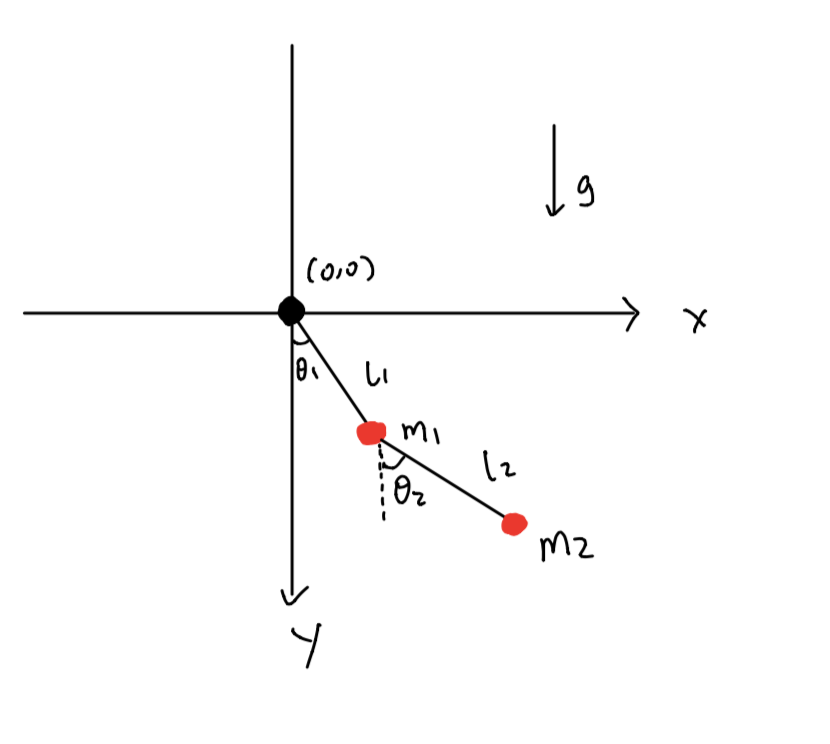
\includegraphics[width=0.6\textwidth]{dp}
\caption{The physics system}
\label{Fig_physics system} 
\end{center}
\end{figure}


\begin{itemize}

\item Gravity: The force that attacts one physical body with mass to another.  
\item Cartesian coordinate system: A coordinate system that specifies each point uniquely in a plane by a set of numerical coordinates, which are the signed distances to the point from two fixed perpendicular oriented lines, measured in the same unit of length. 

\end{itemize}


\subsubsection{Physical System Description}\label{sec_physicsSysDes}
The physics system of Double Pendulum, as shown in (Section~\nameref{Fig_physics system}), includes the following elements:
\begin{itemize}

\item[PS1:] The top mass (with initial angle $\theta_1$)
\item[PS2:] The bottom mass (with initial angle $\theta_2$)
\item[PS3:] The top rob
\item[PS4:] The bottom rob

\end{itemize}

\subsubsection{Goal Statement}\label{sec_goalState}
Given the masses, lengths of robs, initial angles of masses, and the gravitational constant, the goal statements are:
\begin{itemize}

\item[GS\refstepcounter{goalnum}\thegoalnum \label{G_meaningfulLabel}:] Show the graphs of motions of the two masses, namely the graphs of $\theta_1$(t) and $\theta_2$(t).
\end{itemize}

\subsection{Solution Characteristics Specification}\label{sec_solotionSpec}
The instance models that govern Double Pendulum are presented in section~\nameref{sec_instanceModel}. The information to understand the meaning of the instance models and their derivation is also presented, so that the instance models can be verified. 

\subsubsection{Assumptions}\label{sec_assumpt}
This section simplifies the original problem and helps in developing the theoretical models by filling in the missing information for the phisical system. The assumptions refines the scope by providing more detail.
\begin{itemize}

\item[A\refstepcounter{assumpnum}\theassumpnum \label{A_2D}:]
The projectile motion is two-dimensional(2D).  
\item[A\refstepcounter{assumpnum}\theassumpnum \label{A_cartSys}:]
A Cartesian coordinate system is used. 
\item[A\refstepcounter{assumpnum}\theassumpnum \label{A_yGravity}:]
The direction of the y-axis is directly opposite to gravity.  
\item[A\refstepcounter{assumpnum}\theassumpnum \label{A_origin}:]
The double pendulum is attached to the origin.  
\item[A\refstepcounter{assumpnum}\theassumpnum \label{A_neglectCurve}:]
The motion is small enough that the curvature of the Earth can be neglected.  
\item[A\refstepcounter{assumpnum}\theassumpnum \label{A_timeZero}:]
Time starts at zero.  
\item[A\refstepcounter{assumpnum}\theassumpnum \label{A_neglectDrag}:]
Air drag is neglected.  

\end{itemize}


\subsubsection{Theoretical Models}\label{sec_tm}
This section focuses on the general equations and laws that Double Pendulum is based on. 

\noindent
\begin{minipage}{\textwidth}
\renewcommand*{\arraystretch}{1.5}
\begin{tabular}{| p{\colAwidth} | p{\colBwidth}|}
  \hline
  \rowcolor[gray]{0.9}
  Number& T\refstepcounter{theorynum}\thetheorynum \label{T_Newton}\\
  \hline
  Label&\bf Newton's laws of motion\\
  \hline
  Equation& \[F=m * a\]\\
  \hline
  Description & F is the force(N))\newline
                m is the mass(kg)\newline
                a is the acceleration(\( \frac{m}{s^{2}} \))\\
  \hline
  Source &
           \url{https://www.grc.nasa.gov/www/k-12/airplane/newton.html}\\
  \hline
  Ref.\ By & ~\iref{force1}, ~\iref{force2}\\
  \hline
\end{tabular}
\end{minipage}\\

\begin{comment}
\noindent
\begin{minipage}{\textwidth}
\renewcommand*{\arraystretch}{1.5}
\begin{tabular}{| p{\colAwidth} | p{\colBwidth}|}
  \hline
  \rowcolor[gray]{0.9}
  Number& T\refstepcounter{theorynum}\thetheorynum \label{T_AirDrag}\\
  \hline
  Label&\bf Air drag force\\
  \hline
  Equation& \[F_a=\frac{1}{2}c\rho Av^2\]\\
  \hline
  Description & $F_a$ is the air drag force(N))\newline
                c is the dimensionless drag coefficient\newline
                $\rho$ is the density of air (\( \frac{kg}{s^{3}} \)\newline
                A is the cross-sectional area exposed to the air flow($m^2$)\newline
                v is the air flow speed(\( \frac{m}{s}\))\\
  \hline
  Source &
           \url{http://demonstrations.wolfram.com/MotionOfAPendulumInTheWind/}\\
  \hline
  Ref.\ By & \\
  \hline
\end{tabular}
\end{minipage}\\
\end{comment}

\noindent
\begin{minipage}{\textwidth}
\renewcommand*{\arraystretch}{1.5}
\begin{tabular}{| p{\colAwidth} | p{\colBwidth}|}
  \hline
  \rowcolor[gray]{0.9}
  Number& T\refstepcounter{theorynum}\thetheorynum \label{T_Velocity}\\
  \hline
  Label&\bf Velocity\\
  \hline
  Equation& \[v=\frac{dx}{dt}\]\\
  \hline
  Description & v is the velocity(\( \frac{m}{s} \))\newline
                t is the time(s)\newline
                x is the position(m)\\
  \hline
  Source &
           \url{http://wearcam.org/absement/Derivatives_of_displacement.htm}\\
 
  \hline
  Ref.\ By & ~\ddref{velocityx1}, ~\ddref{velocityy1}, ~\ddref{velocityx2},~\ddref{velocityy2}\\
  \hline
\end{tabular}
\end{minipage}\\


\noindent
\begin{minipage}{\textwidth}
\renewcommand*{\arraystretch}{1.5}
\begin{tabular}{| p{\colAwidth} | p{\colBwidth}|}
  \hline
  \rowcolor[gray]{0.9}
  Number& T\refstepcounter{theorynum}\thetheorynum \label{T_Acceleration}\\
  \hline
  Label&\bf Acceleration\\
  \hline
  Equation& \[a=\frac{dv}{dt}\]\\
  \hline
  Description & a is the acceleration(\( \frac{m}{s^{2}} \))\newline
                t is the time(s)\newline
                v is the velocity(\( \frac{m}{s} \))\\
  \hline
  Source &
           \url{http://wearcam.org/absement/Derivatives_of_displacement.htm}\\
  \hline
  Ref.\ By & ~\ddref{accelerationx1},~\ddref{accelerationy1}, ~\ddref{accelerationx2}, ~\ddref{accelerationy2}\\
  \hline
\end{tabular}
\end{minipage}\\




\subsubsection{General Definitions}\label{sec_generalDef}
This section collects the laws and equations that will be used to build the instance models.

\begin{comment}
\noindent
\begin{minipage}{\textwidth}
\renewcommand*{\arraystretch}{1.5}
\begin{tabular}{| p{\colAwidth} | p{\colBwidth}|}
  \hline
  \rowcolor[gray]{0.9}
  Refname& GD\refstepcounter{defnum}\thedefnum \label{sin}\\
  \hline
  Label&\bf Sine Rule\\
  \hline
  Equation& \[\sin\theta = \frac{Opposite}{Hypotenuse}\] \\
  \hline
  Description & 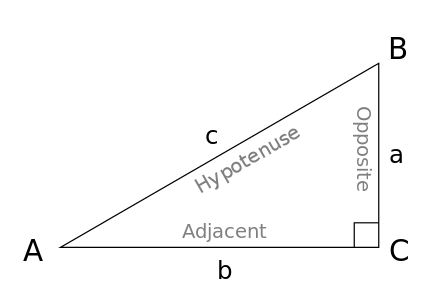
\includegraphics[width=0.3\textwidth, height=30mm]{triangle.png} 

                Opposite is the length of opposite edge(m)\newline
                Hypotenuse is the length of the hypotenuse edge(m)\newline\\
  \hline
  Source &
           \url{https://en.wikipedia.org/wiki/Trigonometry}\\
  \hline
  Ref.\ By & \\
  \hline
\end{tabular}
\end{minipage}\\


\noindent
\begin{minipage}{\textwidth}
\renewcommand*{\arraystretch}{1.5}
\begin{tabular}{| p{\colAwidth} | p{\colBwidth}|}
  \hline
  \rowcolor[gray]{0.9}
  Refname& GD\refstepcounter{defnum}\thedefnum \label{cos}\\
  \hline
  Label&\bf Cosine Rule\\
  \hline
  Equation& \[\cos\theta = \frac{Adjacent}{Hypotenuse}\] \\
  \hline
  Description & 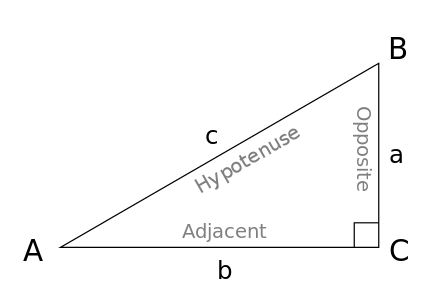
\includegraphics[width=0.3\textwidth, height=30mm]{triangle.png} 

                Adjacent is the length of adjacent edge(m)\newline
                Hypotenuse is the length of the hypotenuse edge(m)\newline\\
  \hline
  Source &
           \url{https://en.wikipedia.org/wiki/Trigonometry}\\
  \hline
  Ref.\ By & \\
  \hline
\end{tabular}
\end{minipage}\\
\end{comment}

% may not have GD

\subsubsection{Data Definitions}\label{sec_dataDef}
This section collects and defines all the data needed to build the instance models. \\

\noindent
\begin{minipage}{\textwidth}
\renewcommand*{\arraystretch}{1.5}
\begin{tabular}{| p{\colAwidth} | p{\colBwidth}|}
\hline
\rowcolor[gray]{0.9}
Number& DD\refstepcounter{datadefnum}\thedatadefnum \label{positionx1}\\
\hline
Label& \bf x-component of initial positions of the top pendulum\\
\hline
Symbol &$x_1$\\
\hline
SI Units & \si{\metre}\\
\hline
Equation&\[x_1=L_1sin\theta_1\]\\
\hline
Description & $x_1$ is the horizontal position of the top pendulum(m)\\
& $L_1$ is the length of the top rod(m)\\
& $\theta_1$ is the angle of the top rod(\si[per-mode=symbol] {\degree})\\
\hline
Sources& https://www.myphysicslab.com/pendulum/double-pendulum-en.html\\
\hline
Ref.\ By & ~\ddref{positionx2}, ~\ddref{velocityx1} \\
\hline
\end{tabular}
\end{minipage}\\

\noindent
\begin{minipage}{\textwidth}
\renewcommand*{\arraystretch}{1.5}
\begin{tabular}{| p{\colAwidth} | p{\colBwidth}|}
\hline
\rowcolor[gray]{0.9}
Number& DD\refstepcounter{datadefnum}\thedatadefnum \label{positiony1}\\
\hline
Label& \bf y-component of initial positions of the top pendulum\\
\hline
Symbol &$y_1$\\
\hline
SI Units & \si{\metre}\\
\hline
Equation&\[y_1=-L_1cos\theta_2\]\\
\hline
Description & $y_1$ is the vertical position of the top pendulum(m)\\
& $L_1$ is the length of the top rod(m)\\
& $\theta_1$ is the angle of the top rod(\si[per-mode=symbol] {\degree})\\
\hline
Sources& https://www.myphysicslab.com/pendulum/double-pendulum-en.html\\
\hline
Ref.\ By & ~\ddref{positiony2}, ~\ddref{velocityy2}\\
\hline
\end{tabular}
\end{minipage}\\

\noindent
\begin{minipage}{\textwidth}
\renewcommand*{\arraystretch}{1.5}
\begin{tabular}{| p{\colAwidth} | p{\colBwidth}|}
\hline
\rowcolor[gray]{0.9}
Number& DD\refstepcounter{datadefnum}\thedatadefnum \label{positionx2}\\
\hline
Label& \bf x-component of initial positions of the bottom mass\\
\hline
Symbol &$x_2$\\
\hline
SI Units & \si{\metre}\\
\hline
Equation&\[x_2=x_1+L_2sin\theta_2\]\\
\hline
Description & $x_2$ is the horizontal position of the bottom pendulum(m)\\
& $L_2$ is the length of the bottom rod(m)\\
& $\theta_2$ is the angle of the botom rod(\si[per-mode=symbol] {\degree})\\
& $x_1$ is the horizontal position of the top pendulum(m)\\
\hline
Sources& https://www.myphysicslab.com/pendulum/double-pendulum-en.html\\
\hline
Ref.\ By & ~\ddref{velocityx2} \\
\hline
\end{tabular}
\end{minipage}\\

\noindent
\begin{minipage}{\textwidth}
\renewcommand*{\arraystretch}{1.5}
\begin{tabular}{| p{\colAwidth} | p{\colBwidth}|}
\hline
\rowcolor[gray]{0.9}
Number& DD\refstepcounter{datadefnum}\thedatadefnum \label{positiony2}\\
\hline
Label& \bf y-component of initial positions of the bottom pendulum\\
\hline
Symbol &$y_2$\\
\hline
SI Units & \si{\metre}\\
\hline
Equation&\[y_2=y_1-L_2cos\theta_2\]\\
\hline
Description & $y_2$ is the vertical position of the bottom pendulum(m)\\
& $L_2$ is the length of the bottom rod(m)\\
& $\theta_2$ is the angle of the botom rod(\si[per-mode=symbol] {\degree})\\
& $y_1$ is the vertical position of the top pendulum(m)\\
\hline
Sources& https://www.myphysicslab.com/pendulum/double-pendulum-en.html\\
\hline
Ref.\ By & ~\ddref{velocityy2} \\
\hline
\end{tabular}
\end{minipage}\\

\noindent
\begin{minipage}{\textwidth}
\renewcommand*{\arraystretch}{1.5}
\begin{tabular}{| p{\colAwidth} | p{\colBwidth}|}
\hline
\rowcolor[gray]{0.9}
Number& DD\refstepcounter{datadefnum}\thedatadefnum \label{velocityx1}\\
\hline
Label& \bf x-component of velocity of the top pendulum\\
\hline
Symbol &${x_1}'$\\
\hline
SI Units & \si[per-mode=symbol] {\metre\per\second}\\
\hline
Equation&\[{x_1}'={\theta_1}'L_1cos\theta_1\]\\
\hline
Description & ${x_1}'$ is the horizontal velocity of the top pendulum(\si[per-mode=symbol] {\metre\per\second})\\
& $L_1$ is the length of the top rod(m)\\
& $\theta_1$ is the angle of the top rod(\si[per-mode=symbol] {\degree})\\
& ${\theta_1}'$ is the angular velocity of the top rod(\si[per-mode=symbol] {\degree\per\second})\\
\hline
Sources& https://www.myphysicslab.com/pendulum/double-pendulum-en.html\\
\hline
Ref.\ By & ~\ddref{accelerationx1}\\
\hline
\end{tabular}
\end{minipage}\\


\noindent
\begin{minipage}{\textwidth}
\renewcommand*{\arraystretch}{1.5}
\begin{tabular}{| p{\colAwidth} | p{\colBwidth}|}
\hline
\rowcolor[gray]{0.9}
Number& DD\refstepcounter{datadefnum}\thedatadefnum \label{velocityy1}\\
\hline
Label& \bf y-component of velocity of the top mass\\
\hline
Symbol &${y_1}'$\\
\hline
SI Units & \si[per-mode=symbol] {\metre\per\second}\\
\hline
Equation&\[{y_1}'={\theta_1}'L_1sin\theta_1\]\\
\hline
Description & ${y_1}'$ is the vertical velocity of the top pendulum(\si[per-mode=symbol] {\metre\per\second})\\
& $L_1$ is the length of the top rod(m)\\
& $\theta_1$ is the angle of the top rod(\si[per-mode=symbol] {\degree})\\
& ${\theta_1}'$ is the angular velocity of the top rod(\si[per-mode=symbol] {\degree\per\second})\\
\hline
Sources& https://www.myphysicslab.com/pendulum/double-pendulum-en.html\\
\hline
Ref.\ By & ~\ddref{accelerationy1}\\
\hline
\end{tabular}
\end{minipage}\\

\noindent
\begin{minipage}{\textwidth}
\renewcommand*{\arraystretch}{1.5}
\begin{tabular}{| p{\colAwidth} | p{\colBwidth}|}
\hline
\rowcolor[gray]{0.9}
Number& DD\refstepcounter{datadefnum}\thedatadefnum \label{velocityx2}\\
\hline
Label& \bf x-component of velocity of the bottom pendulum\\
\hline
Symbol &{$x_2$}'\\
\hline
SI Units & \si[per-mode=symbol] {\metre\per\second}\\
\hline
Equation&\[{x_2}'={x_1}'+{\theta_2}'L_2cos\theta_2\]\\
\hline
Description & {$x_2$}' is the horizontal velocity of the bottom pendulum(m/s)\\
& $L_2$ is the length of the bottom rod(m)\\
& $\theta_2$ is the angle of the botom rod(\si[per-mode=symbol] {\degree})\\
& ${\theta_2}'$ is the angular velocity of the bottom rod(\si[per-mode=symbol] {\degree\per\second})\\
& {$x_1$}' is the horizontal velocity of the top pendulum(m/s)\\
\hline
Sources& https://www.myphysicslab.com/pendulum/double-pendulum-en.html\\
\hline
Ref.\ By & ~\ddref{accelerationx2}\\
\hline
\end{tabular}
\end{minipage}\\

\noindent
\begin{minipage}{\textwidth}
\renewcommand*{\arraystretch}{1.5}
\begin{tabular}{| p{\colAwidth} | p{\colBwidth}|}
\hline
\rowcolor[gray]{0.9}
Number& DD\refstepcounter{datadefnum}\thedatadefnum \label{velocityy2}\\
\hline
Label& \bf y-component of velocity of the bottom pendulum\\
\hline
Symbol &{$y_2$}'\\
\hline
SI Units & \si[per-mode=symbol] {\metre\per\second}\\
\hline
Equation&\[{y_2}'={y_1}'+{\theta_2}'L_2sin\theta_2\]\\
\hline
Description & {$y_2$}' is the vertical velocity of the bottom pendulum(m/s)\\
& $L_2$ is the length of the bottom rod(m)\\
& $\theta_2$ is the angle of the botom rod(\si[per-mode=symbol] {\degree})\\
& ${\theta_2}'$ is the angular velocity of the bottom rod(\si[per-mode=symbol] {\degree\per\second})\\
& {$y_1$}' is the vertical velocity of the top pendulum(m/s)\\
\hline
Sources& https://www.myphysicslab.com/pendulum/double-pendulum-en.html\\
\hline
Ref.\ By & ~\ddref{accelerationy2}\\
\hline
\end{tabular}
\end{minipage}\\

\noindent
\begin{minipage}{\textwidth}
\renewcommand*{\arraystretch}{1.5}
\begin{tabular}{| p{\colAwidth} | p{\colBwidth}|}
\hline
\rowcolor[gray]{0.9}
Number& DD\refstepcounter{datadefnum}\thedatadefnum \label{accelerationx1}\\
\hline
Label& \bf x-component of acceleration of the top pendulum\\
\hline
Symbol &{$x_1$}''\\
\hline
SI Units & \si[per-mode=symbol] {\metre\per\square\second}\\
\hline
Equation&\[{x_1}''=-{{\theta_1}'}^2L_1sin\theta_1+{\theta_1}''L_1cos\theta_1\]\\
\hline
Description & {$x_1$}'' is the horizontal acceleration of the top pendulum(\si[per-mode=symbol] {\degree\per\square\second})\\
& $L_1$ is the length of the top rod(m)\\
& $\theta_1$ is the angle of the top rod(\si[per-mode=symbol] {\degree})\\
& ${\theta_1}'$ is the angular velocity of the top rod(\si[per-mode=symbol] {\degree\per\second})\\
& ${\theta_1}''$ is the angular acceleration of the top rod(\si[per-mode=symbol] {\degree\per\square\second})\\
\hline
Sources& https://www.myphysicslab.com/pendulum/double-pendulum-en.html\\
\hline
Ref.\ By & ~\ddref{accelerationx2}, ~\iref{force1}\\
\hline
\end{tabular}
\end{minipage}\\

\noindent
\begin{minipage}{\textwidth}
\renewcommand*{\arraystretch}{1.5}
\begin{tabular}{| p{\colAwidth} | p{\colBwidth}|}
\hline
\rowcolor[gray]{0.9}
Number& DD\refstepcounter{datadefnum}\thedatadefnum \label{accelerationy1}\\
\hline
Label& \bf y-component of acceleration of the top pendulum\\
\hline
Symbol &{$y_1$}''\\
\hline
SI Units & \si[per-mode=symbol] {\metre\per\square\second}\\
\hline
Equation&\[{y_1}''={{\theta_1}'}^2L_1cos\theta_1+{\theta_1}''L_1sin\theta_1\]\\
\hline
Description & {$y_1$}'' is the vertical acceleration of the top pendulum(\si[per-mode=symbol] {\degree\per\square\second})\\
& $L_1$ is the length of the top rod(m)\\
& $\theta_1$ is the angle of the top rod(\si[per-mode=symbol] {\degree})\\
& ${\theta_1}'$ is the angular velocity of the top rod(\si[per-mode=symbol] {\degree\per\second})\\
& ${\theta_1}''$ is the angular acceleration of the top rod(\si[per-mode=symbol] {\degree\per\square\second})\\
\hline
Sources& https://www.myphysicslab.com/pendulum/double-pendulum-en.html\\
\hline
Ref.\ By & ~\ddref{accelerationy2}, ~\iref{force1} \\
\hline
\end{tabular}
\end{minipage}\\

\noindent
\begin{minipage}{\textwidth}
\renewcommand*{\arraystretch}{1.5}
\begin{tabular}{| p{\colAwidth} | p{\colBwidth}|}
\hline
\rowcolor[gray]{0.9}
Number& DD\refstepcounter{datadefnum}\thedatadefnum \label{accelerationx2}\\
\hline
Label& \bf x-component of acceleration of the bottom pendulum\\
\hline
Symbol &{$x_2$}''\\
\hline
SI Units & \si[per-mode=symbol] {\metre\per\square\second}\\
\hline
Equation&\[{x_2}''={x_1}''-{{\theta_2}'}^2L_2sin\theta_2+{\theta_2}''L_2cos\theta_2\]\\
\hline
Description & {$x_2$}'' is the horizontal acceleration of the bottom pendulum(\si[per-mode=symbol] {\degree\per\square\second})\\
& $L_2$ is the length of the bottom rod(m)\\
& $\theta_2$ is the angle of the bottom rod(\si[per-mode=symbol] {\degree})\\
& ${\theta_2}'$ is the angular velocity of the bottom rod(\si[per-mode=symbol] {\degree\per\second})\\
& ${\theta_2}''$ is the angular acceleration of the bottom rod(\si[per-mode=symbol] {\degree\per\square\second})\\
& {$x_1$}'' is the horizontal acceleration of the top pendulum(\si[per-mode=symbol] {\degree\per\square\second})\\
\hline
Sources& https://www.myphysicslab.com/pendulum/double-pendulum-en.html\\
\hline
Ref.\ By & ~\iref{force2}\\
\hline
\end{tabular}
\end{minipage}\\

\noindent
\begin{minipage}{\textwidth}
\renewcommand*{\arraystretch}{1.5}
\begin{tabular}{| p{\colAwidth} | p{\colBwidth}|}
\hline
\rowcolor[gray]{0.9}
Number& DD\refstepcounter{datadefnum}\thedatadefnum \label{accelerationy2}\\
\hline
Label& \bf y-component of acceleration of the bottom pendulum\\
\hline
Symbol &{$y_2$}''\\
\hline
SI Units & \si[per-mode=symbol] {\metre\per\square\second}\\
\hline
Equation&\[{y_2}''={y_1}''+{{\theta_2}'}^2L_2cos\theta_2+{\theta_2}''L_2sin\theta_2\]\\
\hline
Description & {$y_2$}'' is the vertical acceleration of the bottom pendulum(\si[per-mode=symbol] {\degree\per\square\second})\\
& $L_2$ is the length of the bottom rod(m)\\
& $\theta_2$ is the angle of the bottom rod(\si[per-mode=symbol] {\degree})\\
& ${\theta_2}'$ is the angular velocity of the bottom rod(\si[per-mode=symbol] {\degree\per\second})\\
& ${\theta_2}''$ is the angular acceleration of the bottom rod(\si[per-mode=symbol] {\degree\per\square\second})\\
& {$y_1$}'' is the vertical acceleration of the top pendulum(\si[per-mode=symbol] {\degree\per\square\second})\\
\hline
Sources& https://www.myphysicslab.com/pendulum/double-pendulum-en.html\\
\hline
Ref.\ By & ~\iref{force2}\\
\hline
\end{tabular}
\end{minipage}\\


\subsubsection{Instance Models} \label{sec_instanceModel}
This section transforms the problem defined in section~\nameref{sec_specificSysDes} into one which is expressed in mathematical terms. It uses concrete symbols defined in section~\nameref{sec_dataDef} to replace the abstract symbols in the models identified in section~\nameref{sec_tm} and section~\nameref{sec_generalDef}.\\


\noindent
\begin{minipage}{\textwidth}
\renewcommand*{\arraystretch}{1.5}
\begin{tabular}{| p{\colAwidth} | p{\colBwidth}|}
  \hline
  \rowcolor[gray]{0.9}
  Number& IM\refstepcounter{instnum}\theinstnum \label{force1}\\
  \hline
  Label& \bf calOfForceOnTopPendulum\\
  \hline
  Input&$T_1$, $T_2$, $\theta_1$, $\theta_2$,$m_1$, $g$\\
  \hline
  Output& $m_1{x_1}''$, $m_1{y_1}''$\\
  \hline
  Input Constraints& $\theta_1$,$\theta_2$ $\neq$ 0\\
  \hline
  Output Constraints& None\\
  \hline
  Equation &\[m_1{x_1}''=-T_1sin\theta_1+T_2sin\theta_2\]\\
  &\[m_1{y_1}''=T_1cos\theta_1-T_2cos\theta_2-m_1g\]\\
  \hline
  Description& $m_1{x_1}''$ is the horizontal net force on the top pendulum(N)\\
  & $m_1{y_1}''$ is the veritical net force on the top pendulum(N)\\
  \hline
  Sources& https://www.myphysicslab.com/pendulum/double-pendulum-en.html \\
  \hline
  Ref.\ By & ~\tref{T_Newton}\\
  \hline
\end{tabular}
\end{minipage}\\


\noindent
\begin{minipage}{\textwidth}
\renewcommand*{\arraystretch}{1.5}
\begin{tabular}{| p{\colAwidth} | p{\colBwidth}|}
  \hline
  \rowcolor[gray]{0.9}
  Number& IM\refstepcounter{instnum}\theinstnum \label{force2}\\
  \hline
  Label& \bf calOfForceOnTopPendulum\\
  \hline
  Input&$T_2$, $\theta_2$,$m_2$, $g$\\
  \hline
  Output& $m_2{x_2}''$, $m_2{y_2}''$\\
  \hline
  Input Constraints& $\theta_2$ $\neq$ 0\\
  \hline
  Output Constraints& None\\
  \hline
  Equation &\[m_2{x_2}''=-T_2sin\theta_2\]\\
  &\[m_2{y_2}''=T_2cos\theta_2-m_2g\]\\
  \hline
  Description& $m_2{x_2}''$ is the horizontal net force on the bottom pendulum(N)\\
  & $m_2{y_2}''$ is the veritical net force on the bottom pendulum(N)\\
  \hline
  Sources& https://www.myphysicslab.com/pendulum/double-pendulum-en.html \\
  \hline
  Ref.\ By & ~\tref{T_Newton}\\
  \hline
\end{tabular}
\end{minipage}\\



\noindent
\begin{minipage}{\textwidth}
\renewcommand*{\arraystretch}{1.5}
\begin{tabular}{| p{\colAwidth} | p{\colBwidth}|}
  \hline
  \rowcolor[gray]{0.9}
  Number& IM\refstepcounter{instnum}\theinstnum \label{angularAcc1}\\
  \hline
  Label& \bf calOfAngularAccelerationOfTopPendulum\\
  \hline
  Input&$m_1$,$m_2$,$\theta_1$,$\theta_2$,$L_1$,$L_2$,$g$\\
  \hline
  Output&${\theta_1}''$, ${\theta_2}''$\\
  \hline
  Input Constraints& $\theta_1$,$\theta_2$ $\neq$ 0\\
  \hline
  Output Constraints& None\\
  \hline

  Equation &\[{\theta_1}''=\frac{-g(2m_1+m_2)sin\theta_1-m_2gsin(\theta_1-2\theta_2)-2sin(\theta_1-\theta_2)m_2({{\theta_2}'}^2L_2+{{\theta_2}'}^2L_1cos(\theta_1-\theta_2)}{L_1(2m_1+m_2-m_2cos(2\theta_1-2\theta_2))}\]\\
  &\[{\theta_2}''=\frac{2sin(\theta_1-\theta_2)({\theta_1}'L_1(m1+m2)+g(m_1+m_2)cos(\theta_1)+{(\theta_2}')^2L_2m_2cos(\theta_1-\theta_2}{L_2(2m_1+m_2-m_2cos(2\theta_1-2\theta_2))}\]\\

  \hline
  Description& $m_2{x_2}''$ is the horizontal net force on the bottom pendulum(N)\\
  & $m_2{y_2}''$ is the veritical net force on the bottom pendulum(N)\\
  \hline
  Sources& https://www.myphysicslab.com/pendulum/double-pendulum-en.html \\
  \hline
  Ref.\ By & ~\iref{force1}, ~\ddref{accelerationx1}, ~\ddref{accelerationy1}, ~\ddref{accelerationx2},~\ddref{accelerationy2}\\
  \hline
\end{tabular}
\end{minipage}\\




\subsubsection{Input Data Constraints}\label{sec_inputDataCons}

Table ~\nameref{TblInputVar} shows the data constraints on the input output
variables. The column for physical constraints gives the physical limitations
on the range of values that can be taken by the variable. The column for
software constraints restricts the range of inputs to reasonable values. The
software constraints will be helpful in the design stage for picking suitable
algorithms. The constraints are conservative, to give the user of the model the
flexibility to experiment with unusual situations. The column of typical values
is intended to provide a feel for a common scenario. 

\begin{table}[H]
  \caption{Input Variables} \label{TblInputVar}
  \renewcommand{\arraystretch}{1.2}
\noindent \begin{longtable*}{l l l l c} 
  \toprule
  \textbf{Var} & \textbf{Physical Constraints} & \textbf{Software Constraints} &
                             \textbf{Typical Value} & \textbf{Uncertainty}\\
  \midrule 
  $m_1$ & $m_1 > 0$ & - & \si[per-mode=symbol] {\kilogram} & 10\%
  \\
  $m_2$ & $m_2 > 0$ & - & \si[per-mode=symbol] {\kilogram} & 10\%
  \\
  $L_1$ & $L_1 > 0$ & - & \si[per-mode=symbol] {\metre} & 10\%
  \\
  $L_2$ & $L_2 > 0$ & - & \si[per-mode=symbol] {\metre} & 10\%
  \\
  $\theta_1$ & $\theta_1 \neq 0$ & - & \si[per-mode=symbol] {\degree} & 10\%
  \\
  $\theta_2$ & $\theta_2 \neq 0$ & - & \si[per-mode=symbol] {\degree} & 10\%
  \\
  $g$ & $g > 0$ & - & \si[per-mode=symbol] {\newton\per\kilogram} & 10\%
  \\
  \bottomrule
\end{longtable*}
\end{table}

\subsubsection{Properties of a Correct Solution}\label{sec_corSol}
Table ~\nameref{TblOutputVar} shows the data constraints on the outout variables. The column for physical constraints gives the physical limitations on the range of values that can be taken by the variable.

\begin{table}[!h]
\caption{Output Variables} \label{TblOutputVar}
\renewcommand{\arraystretch}{1.2}
\noindent \begin{longtable*}{l l} 
  \toprule
  \textbf{Var} & \textbf{Physical Constraints} \\
  \midrule 
  ${\theta_1}''$ & ${\theta_1}'' \neq 0$\\
  ${\theta_2}''$ & ${\theta_2}'' \neq 0$\\
  \bottomrule
\end{longtable*}
\end{table}

\section{Requirements}\label{sec_req}
This section provides the functional requirements, the business tasks that the
software is expected to complete, and the nonfunctional requirements, the
qualities that the software is expected to exhibit.

\subsection{Functional Requirements}\label{sec_funReq}
This section provides the functional requirements, the tasks and behaviours that the software is expected to complete. \\
\noindent \begin{itemize}

\item[R\refstepcounter{reqnum}\thereqnum \label{R_Inputs}:] 
Input the values from 
\item[R\refstepcounter{reqnum}\thereqnum \label{R_VarifyInputs}:]  
Check the entered input values to ensure that they do not exceed the data constraints mention in section~\nameref{sec_inputDataCons}
\item[R\refstepcounter{reqnum}\thereqnum \label{R_Calculate}:] Calculate the equation for the following values: $\theta_1$(t) (from ) and $\theta_1$(t) (from ).

\item[R\refstepcounter{reqnum}\thereqnum \label{R_Output}:] Output graphs of $\theta_1$(t) (from ) and $\theta_1$(t) (from ).

\end{itemize}

\subsection{Nonfunctional Requirements}\label{sec_nfr}
This section provides the non-functional requirements, the qualities that the software is expected to exhibit.


\noindent \begin{itemize}

\item[NFR\refstepcounter{reqnum}\thereqnum \label{NFR_Correct}:] 
The outputs of the code have the properties described in section~\nameref{sec_corSol}.
\item[NFR\refstepcounter{reqnum}\thereqnum \label{NFR_Verifiable}:]  
The code is tested with complete verification and validation plan.
\item[NFR\refstepcounter{reqnum}\thereqnum \label{R_Reusable}:]
The code is modularized. 
\item[NFR\refstepcounter{reqnum}\thereqnum \label{R_Maintainable}:]
The traceability between requirements, assumptions, theoretical models, general definitions, data definitions, instance models, likely changes, unlikely changes, and modules is completely recorded in traceability matrices in teh SRS and module guide. 
\item[NFR\refstepcounter{reqnum}\thereqnum \label{R_Portable}:]
The code is able to be run in different environments. 
The code is modularized.
\end{itemize}

\section{Likely Changes}\label{sec_likelyChanges}
\noindent \begin{itemize}

\item[LC\refstepcounter{lcnum}\thelcnum\label{LC_airdrag}:] Air drag might be considered.(Ref. by~\aref{A_neglectDrag})

\end{itemize}

\section{Unlikely Changes}\label{sec_unlikelyChanges}
\noindent \begin{itemize}

\item[LC\refstepcounter{lcnum}\thelcnum\label{LC_units}:] The units used will not likely to be changed.   

\end{itemize}

\section{Traceability Matrices and Graphs}\label{sec_traceMatricesGraph}
\afterpage{
\begin{landscape} 
\begin{table}[H]
\centering
\begin{tabular}{|c|c|c|c|c|c|c|c|c|c|c|c|c|c|c|c|c|c|c|c|}
\hline
  & \aref{A_2D}& \aref{A_cartSys}& \aref{A_yGravity}& \aref{A_origin}& \aref{A_neglectCurve}& \aref{A_timeZero}& \aref{A_neglectDrag}\\
\hline
\tref{T_Newton}        & & & & & & &\\ \hline
\tref{T_Velocity}        & & & & & & & \\ \hline
\tref{T_Acceleration}        & & & & & & & \\ \hline
\ddref{positionx1}           & & & & & & &  \\ \hline
\ddref{positiony1}         & & & & & & & \\ \hline
\ddref{positionx2}    & & & & & & & \\ \hline
\ddref{positiony2}     & & & & & & & \\ \hline
\ddref{velocityx1}       & & & & & & & \\ \hline
\ddref{velocityy1}        & & & & & & & \\ \hline
\ddref{velocityx2}        & & & & & & & \\ \hline
\ddref{velocityy2}        & & & & & & & \\ \hline
\ddref{accelerationx1}        & & & & & & & \\ \hline
\ddref{accelerationy1}        & & & & & & & \\ \hline
\ddref{accelerationx2}        & & & & & & & \\ \hline
\ddref{accelerationy2}        & & & & & & & \\ \hline
\iref{force1}         & X&X &X & &X & & X\\ \hline
\iref{force2}      & X&X &X & &X & & X\\ \hline
\iref{angularAcc1}       & X&X &X &X &X & & \\ \hline
\lcref{LC_airdrag}    & & & & & & & X\\ \hline
\lcref{LC_units}    & & & & & & & \\ 
\hline
\end{tabular}
\caption{Traceability Matrix Showing the Connections Between Assumptions and Other Items}
\label{Table:A_trace}
\end{table}
\end{landscape}
}

\begin{table}[H]
\centering
\begin{adjustbox}{width=1\textwidth}
\small
\begin{tabular}{|c|c|c|c|c|c|c|c|c|c|c|c|c|c|c|c|c|c|c|c|c|c|c|c|c|c|c|c|c|c|c|c|c|c|}
\hline        
  & \tref{T_Newton} & \tref{T_Velocity} & \tref{T_Acceleration} & \ddref{positionx1} &\ddref{positiony1} & \ddref{positionx2} & \ddref{positiony2} & \ddref{velocityx1} & \ddref{velocityy1} & \ddref{velocityx2} & \ddref{velocityy2} & \ddref{accelerationx1} & \ddref{accelerationy1} & \ddref{accelerationx2} & \ddref{accelerationy2} & \iref{force1} & \iref{force2} & \iref{angularAcc1} & \lcref{LC_airdrag} & \lcref{LC_units} \\
\hline
\tref{T_Newton}        &&&&&&&&&&&&&&&&X&X&&&\\ \hline
\tref{T_Velocity}        &&&&&&&&X&X&X&X&&&&&&&&&\\ \hline
\tref{T_Acceleration}        &&&&&&&&&&&&X&X&X&X&&&&&\\ \hline
\ddref{positionx1}           &&&&&&X&&X&&&&&&&&&&&&\\ \hline
\ddref{positiony1}         &&&&&&&X&&&&X&&&&&&&&&\\ \hline
\ddref{positionx2}    &&&&&&&&&&X&&&&&&&&&& \\ \hline
\ddref{positiony2}     &&&&&&&&&&&X&&&&&&&&&\\ \hline
\dref{velocityx1}       &&&&&&&&&&&&X&&&&&&&&\\ \hline
\dref{velocityy1}        &&&&&&&&&&&&&X&&&&&&&\\ \hline
\dref{velocityx2}        &&&&&&&&&&&&&&X&&&&&&\\ \hline
\dref{velocityy2}       &&&&&&&&&&&&&&&X&&&&&\\ \hline
\dref{accelerationx1}        &&&&&&&&&&&&&&X&&X&&&& \\ \hline
\dref{accelerationy1}        &&&&&&&&&&&&&&&X&X&&&&\\ \hline
\dref{accelerationx2}       &&&&&&&&&&&&&&&&&X&&&\\ \hline
\dref{accelerationy2}       &&&&&&&&&&&&&&&&&X&&&\\ \hline
\iref{force1}        &X&&&&&&&&&&&&&&&&&&&\\ \hline
\iref{force2}      &X&&&&&&&&&&&&&&&&&&&\\ \hline
\iref{angularAcc1}       &X&&&&&&&&&&&X&X&X&X&&&&&\\ \hline
\lcref{LC_airdrag}    &&&&&&&&&&&&&&&&&&&&\\ \hline
\lcref{LC_units}    &&&&&&&&&&&&&&&&&&&&\\ 
\hline
\end{tabular}
\end{adjustbox} 
\caption{Traceability Matrix Showing the Connections Between Items of Different Sections}
\label{Table:trace}
\end{table}


\begin{table}[H]
\centering
\begin{tabular}{|c|c|c|c|c|c|c|c|}
\hline
  & \iref{force1}& \iref{force2}& \iref{angularAcc1}& \rref{R_Inputs}& \rref{R_VarifyInputs} &  \rref{R_Calculate} & \rref{R_Output}\\
\hline
\iref{force1}            &&&&&X&X&X \\ \hline
\iref{force2}            &&&&&X&X&X\\ \hline
\iref{angularAcc1}         &&&&&X&X&X\\ \hline
\rref{R_Inputs}         &X&X&X&&&&\\ \hline
\rref{R_VarifyInputs}         &X&X&X&&&&\\ \hline
\rref{R_Calculate}     &X&X&X&&&&\\ \hline
\rref{R_Output}    &X&X&X&&&&\\  
\hline
\end{tabular}
\caption{Traceability Matrix Showing the Connections Between Requirements and Instance Models}
\label{Table:R_trace}
\end{table}




\section{Values of Auxiliary Constants}\label{sec_auxConst}

NA.
\end{document}